\documentclass[11pt]{article}

%%%%%%%%%%%%%%%%%%%%%%%%%%%%%%%%%%%%%
%		Packages
%%%%%%%%%%%%%%%%%%%%%%%%%%%%%%%%%%%%%
\usepackage{graphicx}
\usepackage{geometry}
 \geometry{ a4paper,
 total={170mm,257mm},
 left=20mm,
 top=20mm }
\usepackage{multicol}
\usepackage{enumitem}
\usepackage[linesnumbered,ruled]{algorithm2e}
\usepackage{multirow}
\usepackage{arydshln}
\usepackage{mathtools}
\usepackage{cite}
\usepackage{float} % privides the H option
\usepackage{eurosym}
\usepackage{amsmath}
\usepackage{mathptmx,mathtools}
\usepackage{subcaption}
\usepackage[utf8]{inputenc}
\usepackage[english]{babel}
\allowdisplaybreaks


\begin{document}

\title{Improved Ramping Behaviour Analysis model \\ for scenario generation using Markov-chain}
\author{
        Sambeet Mishra, Esin Oren and Ivo Palu\\
    Tallinn University of Technology, Tallinn, Estonia
}
\date{\today}
\maketitle

\begin{abstract}
Power generation from wind farm varies with time. This power swing increases the challenges in full utilization of the resource. The power system planner need to ensure supply of power on demand. Accurate estimation of power production from non-dispatchable resources such as wind is essential for the planner to ensure the supply-demand balance and reserve power capacity. 
This paper investigates the power swings and introduces improved ramping behavior analysis model namely RBA$_\theta$. The objective of the proposed model is to quantify the variations as events. Each event is described through parameters- Up-ramp, Down-ramp, Peak, Frequency and Persistence. For this investigation, wind power production data is obtained from a wind farm containing 8 turbines. The data is normalized and scaled between 0 and 1. The geographical location of are synthesized from coastal region of Estonia. In first step, the events are extracted from the time-series wind power production data. In step two, the rain-flow counting algorithm is used to identify the cycles in the time-series data. These cycles explain if a noticeable pattern occurs multiple times in the data.  
Subsequently in step 3, a spatial Markov chain is implemented that takes the location as input and produce a matrix of transition probabilities. Then in step 4, the sequence of events are predicted with reference to time. Subsequently in final step, the transition matrices containing spatial information and time-series events are combined to generate scenarios that are- most likely, least likely and probable. The scenarios are generated for a long term and short term period. A comparative analysis between temporal scenarios and spatio-temporal scenarios is presented to outline the importance of the proposed method. 
\end{abstract}



\begin{description}[noitemsep]
\item[Nomenclature] 
\item[RBA]	Ramping Behaviour Analysis
\end{description}


\section{Introduction} \label{sec:intro}

Wind energy is stochastic in nature due the flow of wind is a product of multiple natural phenomenon. 
When there is a small penetration of wind into the power systems, the uncertain behaviour of the wind power generation is treated as just another uncertainty on the demand side. Moreover, the conventional power stations covering this variability, require additional energy and reduce the environmental benefits. Forecasting is one of the many possible solutions to this problem, as well as an interconnected grid, energy storage technologies, demand-side management such as electric vehicles. Forecasting aims to model the uncertainties inherited by the grid through wind power production and thus is a necessary and cost-effective element for the optimal integration of wind power into energy systems. However, forecasting is never accurate and literature suggests providing bounds for the forecasts or confidence intervals.
Wind power is intermittent by nature due to weather. A wind power ramp event can be termed as a sudden change in the output power over a set threshold. Mathematically, the absolute difference between power produced $P_t$ in time $t$ and $(t + \Delta \; t)$ that is above the set threshold $\overline{P}$ is a ramp event as in \eqref{eqn:rba}. However the threshold value is subjective. 

\begin{equation} \label{eqn:rba}
    | P_{(t + \Delta \; t)} - P_t | > \overline{P}
\end{equation}

\par
The system operator (SO) has to keep the system balanced i.e, the generation must meet the demand at each point in time. Wind ramp events can be positive or negative based on the generation swings. If positive, then the wind turbine has to shut down to avoid accidents or damage to the system whereas if the swing is negative the SO has to find a replacement to mitigate the demand. From economical point of view, both the energy not used and energy from an alternative resource are crucial. 
Each wind farm forecasts wind speed and power production from historical data over time with an objective to determine potential investment and operations. In long-term forecasting the events become insignificant due to time-stretch while in short-term forecasting of events are more accurate. Furthermore, the time interval $\Delta \; t$ is typically 10 minutes for ramp events. The $\overline{P}$ is either set to an absolute value for a wind park or a certain percentage of the generation depending on the installed capacity. The problem with this practice is that the peak generation capacity varies through seasons and turbine maintenance or new installations. Although the threshold is subjective to peculiarities of a wind park, the methods to classify ramp events is generic. This work draws its focus on the procedure to detect ramp events. In addition demonstrates the application on real data from wind park. 
\subsection{Previous work} \label{previous work}

There are many studies in the literature on characteristics of wind power, correlations of wind and wind power, forecasting wind and wind power output, scenario generation. In \cite{bianco2016wind} the authors proposed a model to forecast ramp events as well. They modelled observed wind speeds into forecast models and converted this into power forecasts with the help of the power curve of the wind turbines. It suggests that the same method could be implemented for solar power plants. Another noteworthy one is a model-free forecast generation implemented with Generative Adversarial Networks (GAN). GANs have two de-convolutional, one that starts by generating random data and the out discriminates whether its input is coming from the generator or historical data. These two neural networks play a Nashville game while giving feedback to each other, both getting better over time until the generator generates data that is almost like a forecast so that the discriminator can not discriminate any more. \cite{cui2016optimized} proposed a probabilistic forecasting method, utilizing a Neural Network(NN) to generate possible future scenarios, employing an objective function based on cumulative distribution functions and auto-correlation functions to train the NN, primarily teaching it their distribution. Again another \cite{karatepe2013wind} proposed a model to synthesized wind speed scenarios based on statistical parameters of wind and Markov chains. In contrast, \cite{kaut2014copula} proposes a new heuristic to generate scenarios that use copulas instead of common correlation functions. \cite{ArticleNo1,ArticleNo2} introduced the terminology for identification of ramp events, ramping behaviour analysis(RBA), which comprises the perspective used in this study. They also filtered and extracted events, and clustered them into groups. More studies have been performed on identifying ramp events in \cite{bossavy2013forecasting, bossavy2013novel, cui2016optimized}. 

\subsection{Contribution of this paper}
This paper investigates the variations in the wind power generation and contributes to the variation quantification and prediction methodology. The proposed model can be used for operational planning of wind farms and injection of wind power into the system.
RBA$_\theta$ is a novel method considering spatio-temporal information of power variations. The proposed model has the following advantages over the existing models: 
\begin{description}
\item[Cleaning the data] Prediction of discrete time-series data may contain some irregularities in form of noise. Therefore, pre-processing the data and removing the noise content is essential for accurate prediction. 
\item[Spatial information] The location of the turbines has a significant impact of the production. Therefore, RBA$_\theta$ takes into account the spatio-temporal information: location of turbines and power production through a markovian transition matrix. This matrix has transition probabilities with likelihood from one state to another state.
\item[Prediction of events] The operational planning for a wind farm plans for responses to significant events such as high power generation and very low power generation. As a consequence, generating the scenarios for the events that might occur based on the historical pattern facilitates the planning.
\end{description}
 


\section{Modelling Ramping Behaviour Analysis Algorithm} \label{sec:model}

The wind power variations are classified by wind the ramp events. The RBA (Ramping Behaviour Analysis) is an algorithm that determines ramp events based on peak power. This algorithm has four components: rise time, fall time, ramp-up rate and ramp-down rate. The graphical representation in fig. \ref{fig:rba} describes a ramp event and the associated components. The angle ($\theta$) is with reference to the peak point for both up-ramp and down-ramp events. The persistence describes the amount of time the peak event persists. The rise-time and fall-time are presented as $\Delta \; t^{up}$ and $\Delta \; t^{down}$ respectively.

  \begin{figure}[H]
    \centering
    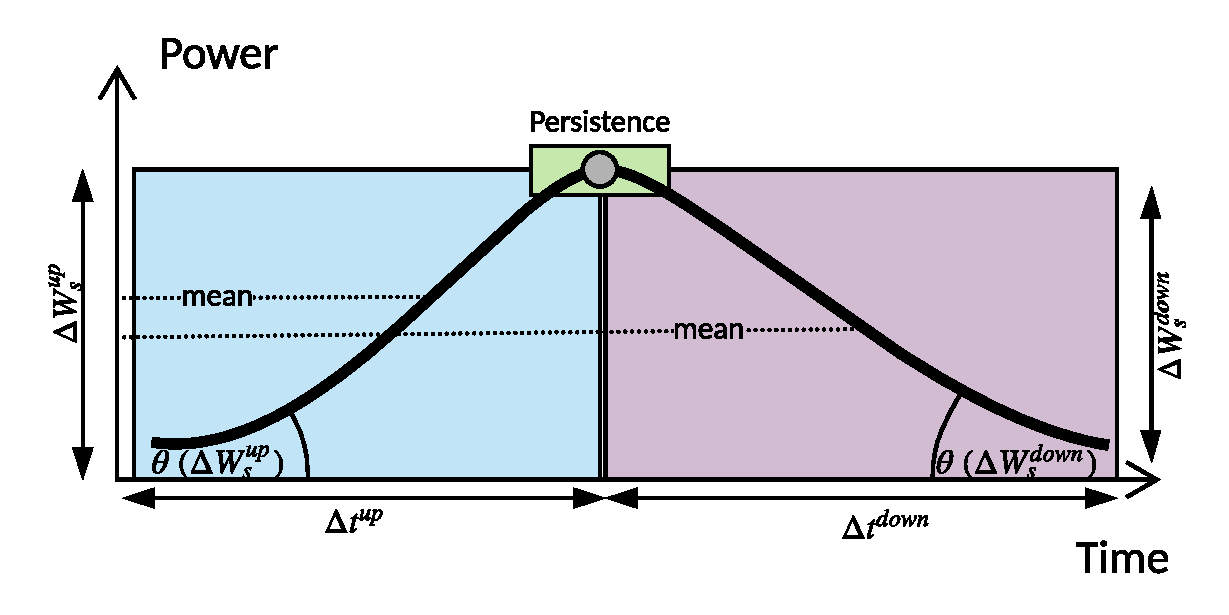
\includegraphics[width=.8\textwidth]{./sec/fig/RBA_new.pdf}
    \caption{Wind ramp event classification}
    \label{fig:rba}
\end{figure}


\subsection{Wind power data}
The data is obtained from the wind park with hourly time resolution. All data points coincide with each other date and time-wise for each turbine. Fig. \ref{fig:wind_data} presents the power output from the wind park for 8760 hours. The data has certainly many power swings and it can be seen more clearly when a smaller time-window is chosen. However, the data is demonstrated with a top-view to show the pattern in seasons. For example, the winter season has dense power power production in comparison to lighter one in summer. 


  \begin{figure}[!htbp]
    \centering
    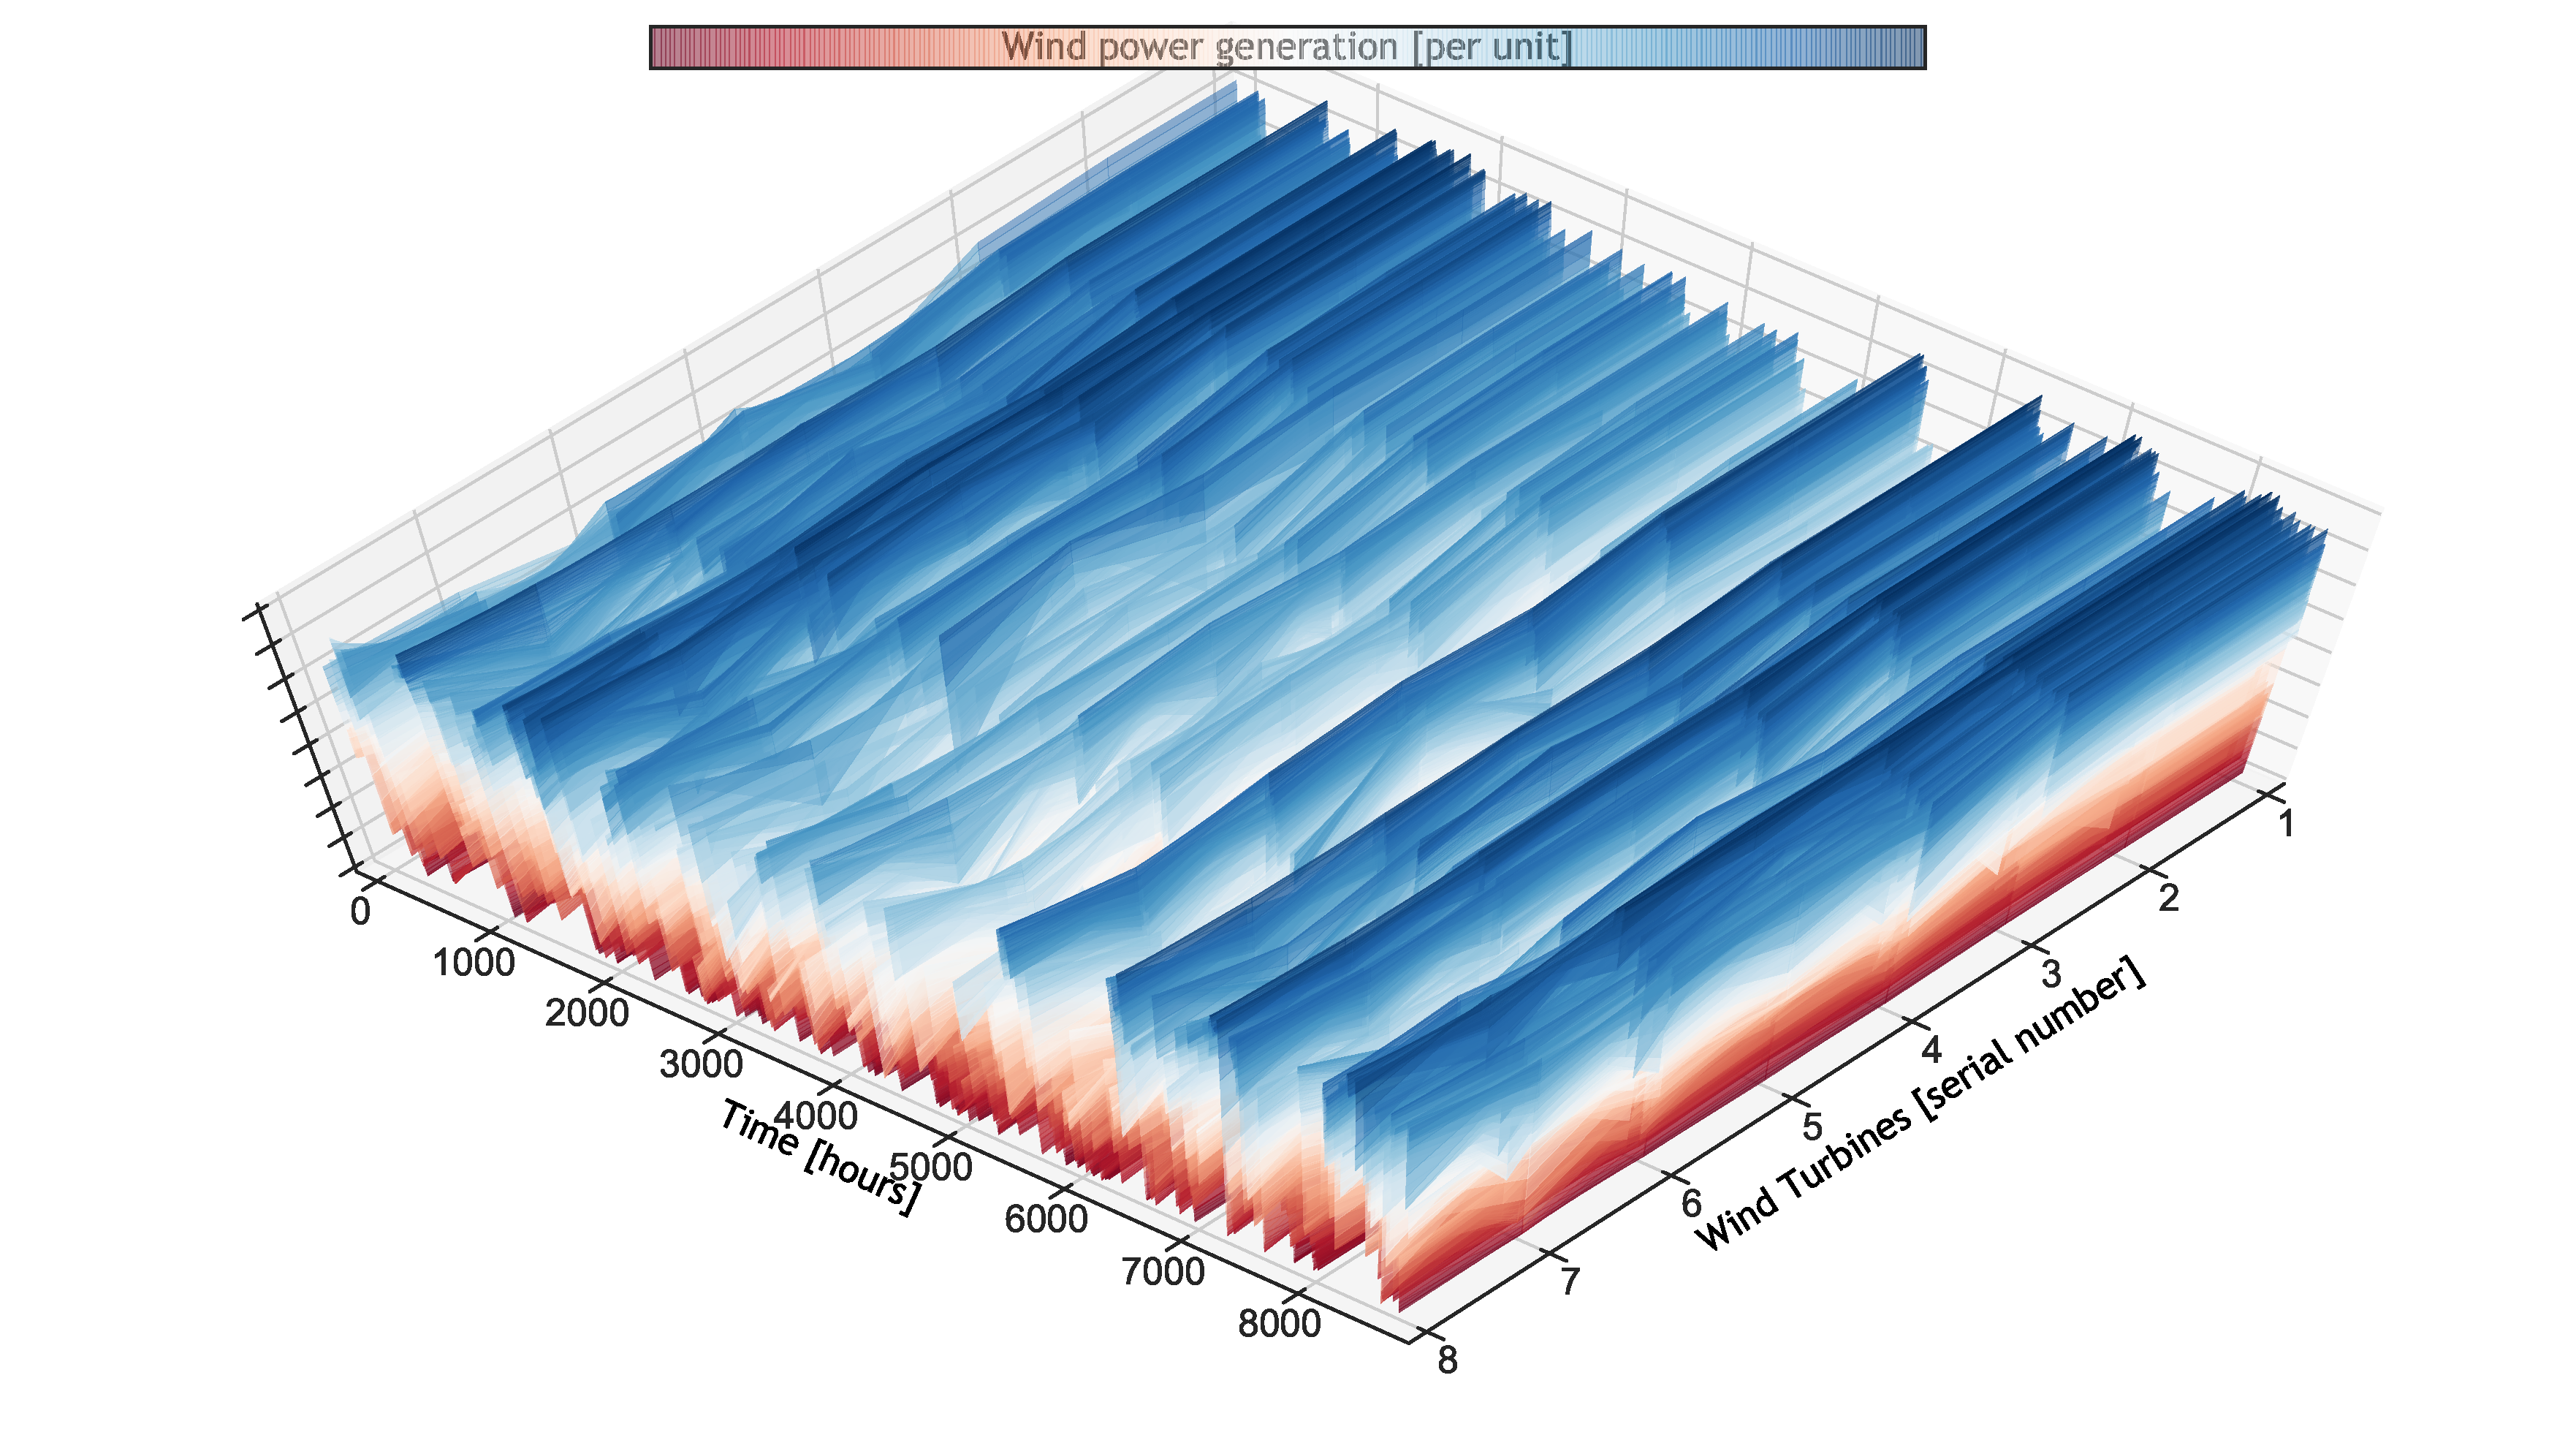
\includegraphics[width=\textwidth]{./sec/fig/wind_data.pdf}
    \caption{Wind power generation from Palidiski wind farm}
    \label{fig:wind_data}
\end{figure}

wind production of a turbine is expressed through capacity factor: the ratio between the net power generation and the calibrated  as in \( \displaystyle \frac{P_{net}}{P_{rated}} \). The data are registered with a time stamp, however the relation between two subsequent observation is not. Again, the degree of noise content that is inherent to the data is substantial for event detection. For example one outlier could either be a significant event. Thus raw data is smoothed through different smoothing techniques to capture the significant events. 

\begin{figure}[!htbp]
 \centering
    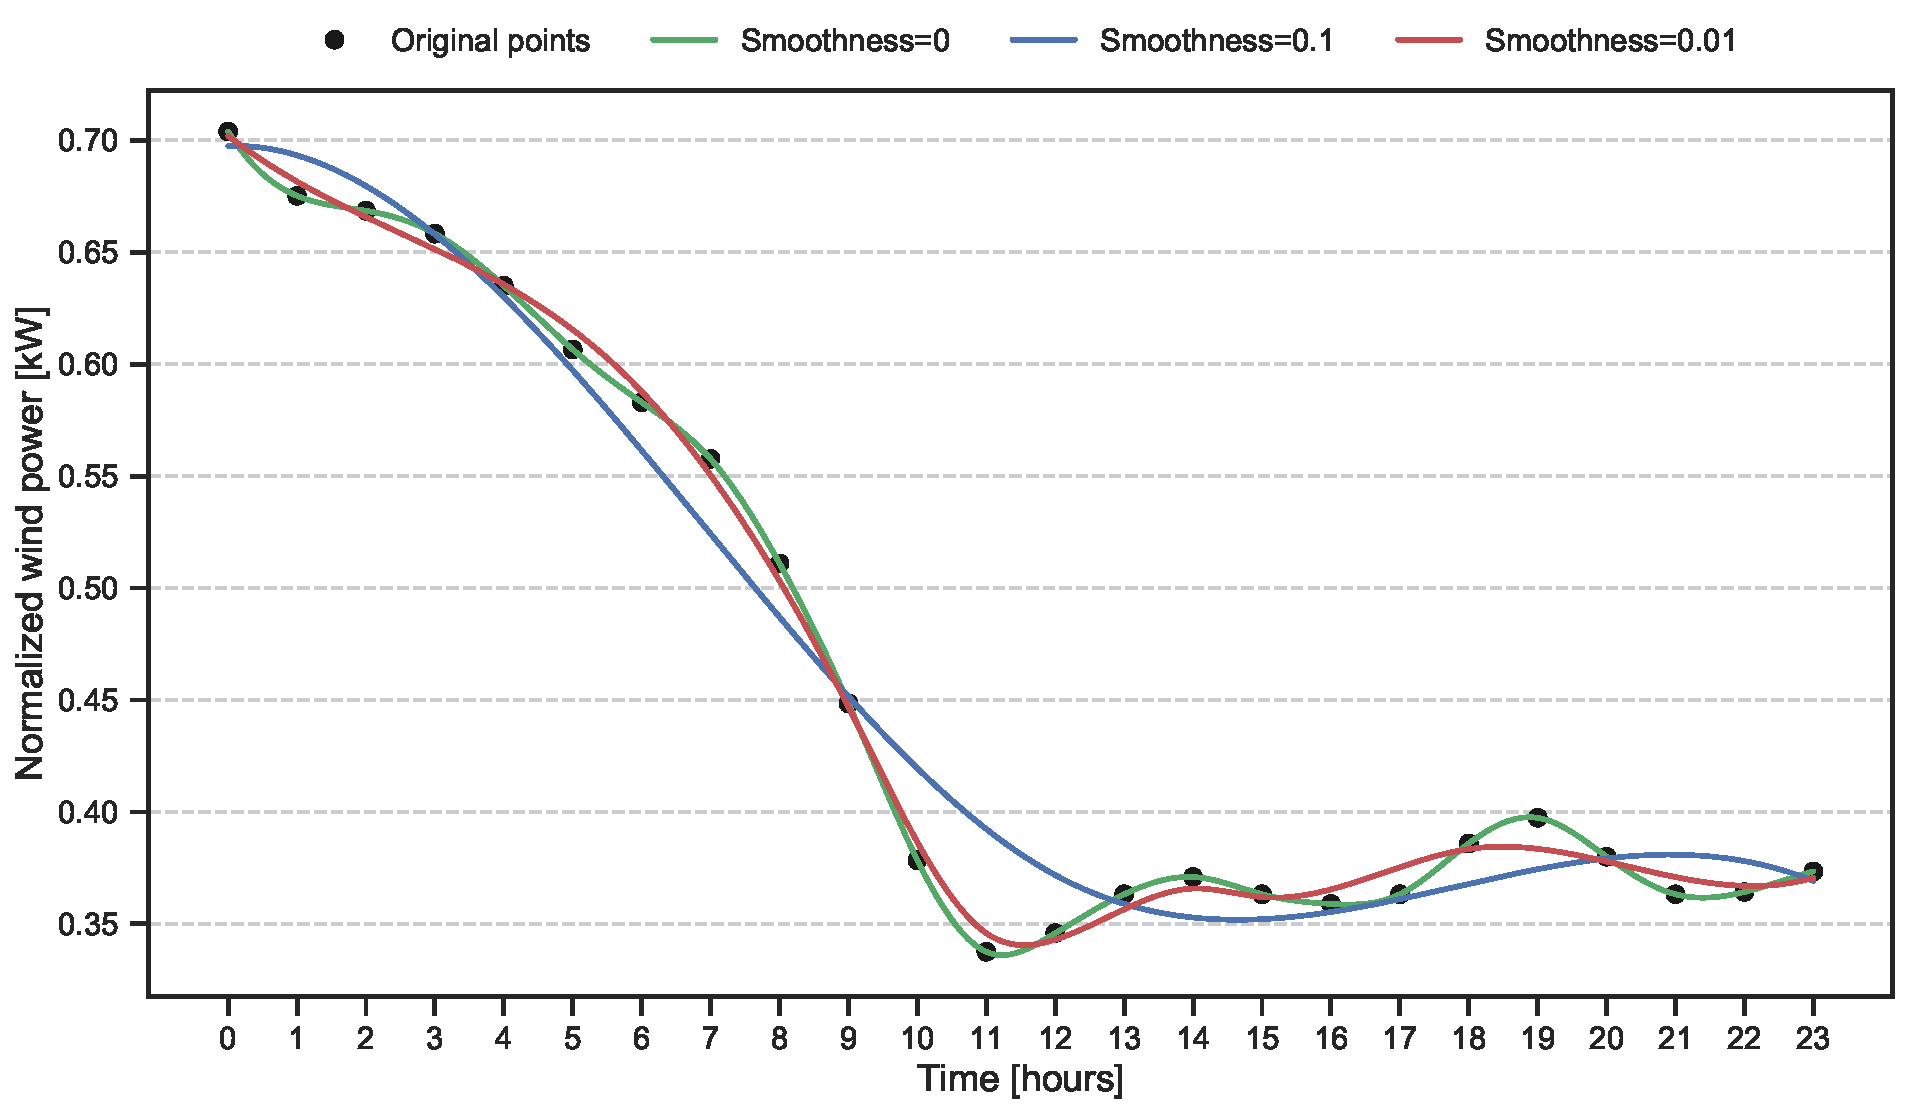
\includegraphics[width=0.8\textwidth]{./sec/fig/Splined_Plot.pdf}
    \caption{Wind power data smoothing using cubic spline smoothing technique}
    \label{fig:data_splined}
\end{figure}

The wind power production data from the wind farm is pre-processed to smoothing technique. A cubic spline method is chosen that is a special case of spline interpolation. In \eqref{eq:spline} presents the $S_i$ cubic spline function. Subsequently the coefficients are obtained starting from $z_0$ and then using the recurrence relation. This technique has smaller error than Newton polynomial and Lagrange polynomial \cite{de1978practical}. In fig. \ref{fig:data_splined} the original data and a comparison between smoothness 0, 0.1 and 0.01 for a 24 hour period is presented. It is evident that smoothness 0.01 is very close to the original trend in the wind power data. 

\begin{subequations} \label{eq:spline}
\begin{align}
S_i (x) & = y_i + z_i (x - x_i) + \frac{z_{i+1} - z_i}{2 * (x_{i+1} - x_i)} (x-x_i)^2  \\
z_{i+1} & = - z_i + 2 * \frac{y_{i+1} - y_i}{x_{i+1} - x_i}
\end{align}
\end{subequations}

%Exponential moving average filter technique is used for smoothing the data as in \eqref{eq:ma}. Here $f, c, p, w$ stands for exponential moving average, current value, previous value and $w=2/(N+1)$ weight factor wherein $N$ is number of periods respectively. The results are presented in the subsequent publication \cite{ArticleNo1}.
%
%\begin{equation}\label{eq:ma}
%    f(c) = \big[ \{ c - f(p) \} w \big] + f(p)
%\end{equation}

A given function or signal can be transformed  from time to frequency domain and other way round. The frequency domain transforms the linear differential to algebraic equations which are easy to solve. Furthermore, the latter provides qualitative behavior of the system: such as bandwidth, frequency response, gain, phase shift, power spectral density, eigenvalues to name a few. The focus on this thesis is limited to spectral density and FFT (Fast Fourier transformation). The Fourier transform of a function contains all the information about the original signal, and with this information, it is possible to reconstruct the function entirely by an inverse Fourier transform. This information includes amplitude and phase of each frequency present in the function. 
The Fourier transform of a discrete-time signal $x[n], n=0,..,N$ is called the discrete-time Fourier transform (DTFT), which provides a mathematical approximation of the full integral solution, and yields a periodic frequency spectrum. The DTFT of the sequence $x[n]$ denoted in  \eqref{eq:filter1} is a function of a continuous frequency variable $\omega$ and $X(e^j\omega )$ and is always periodic with period $2 \pi$. And \eqref{eq:filter2} represents the inverse DTFT of $x[n]$. DFT (Discrete Fourier Transform) can be obtained from the DTFT by evaluating through a discrete set of equally spaced frequencies \cite{mcclellan2003signal}. 

\begin{subequations}
\begin{align} 
\centering
X( e^{j\omega} ) & = \sum_{n=- \infty}^{\infty} x[n] e^{-j \omega n} \label{eq:filter1}\\
x[n]  & = \frac{1}{2 \pi} \int_{- \pi}^{\pi} X( e^{j\omega} ) e^{-j \omega n} d \omega \label{eq:filter2}
\end{align}
\end{subequations}

A finite number of samples are selected to determine the spectrum. Then a window is generated by a multiplication of $x[n]$ by another sequence $w[n]$. Blackman window is selected for the study \cite{agarwal2014mathematical}. A time-domain representation of the same is presented in \eqref{eq:fd} where $N$ is the \textit{length} of Blackman window.

\begin{align} \label{eq:fd}
    w(n) = 0.42 - 5 \cos \left( \frac{2 \pi n}{N-1} \right) +0.88 \cos \left( \frac{4 \pi n}{N - 1} \right) \qquad \forall \; 0 \leq n \leq (M-1) 
\end{align}

\[
 M =
  \begin{cases}
    N/2       & \quad \text{if } N \text{ is even}\\
    (N+1)/2  & \quad \text{if } N \text{ is odd}
  \end{cases}
\]


\begin{figure}[!htbp]
 \centering
    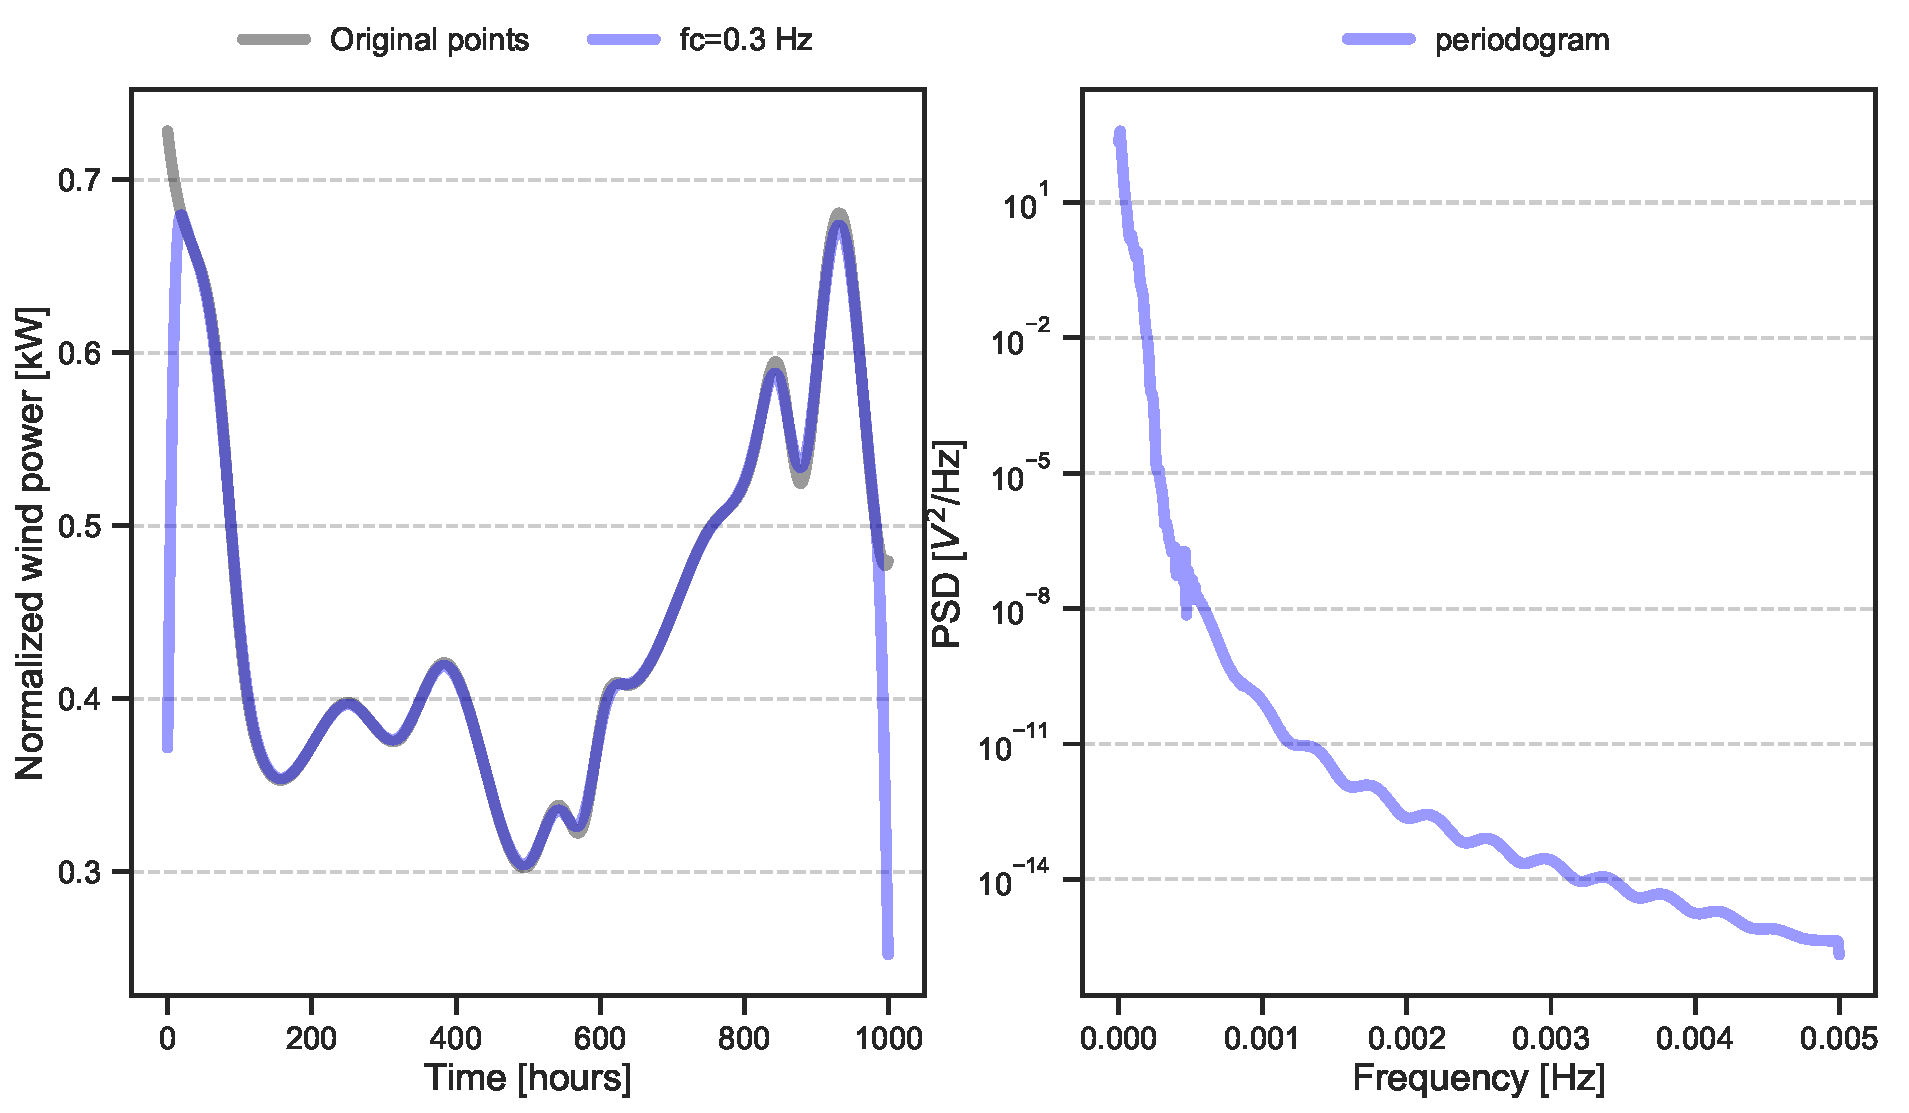
\includegraphics[width=0.8\textwidth]{./sec/fig/Time-to-freq_plot.pdf}
    \caption{Frequency domain transformation: (A) filtered data with 0.3 Hz cut-off frequency (B) periodogram plot showing power spectral density}
    \label{fig:fft}
\end{figure}


%  \begin{figure}[!ht]
%\centering
%\begin{subfigure}{.5\textwidth}
%  \centering
%  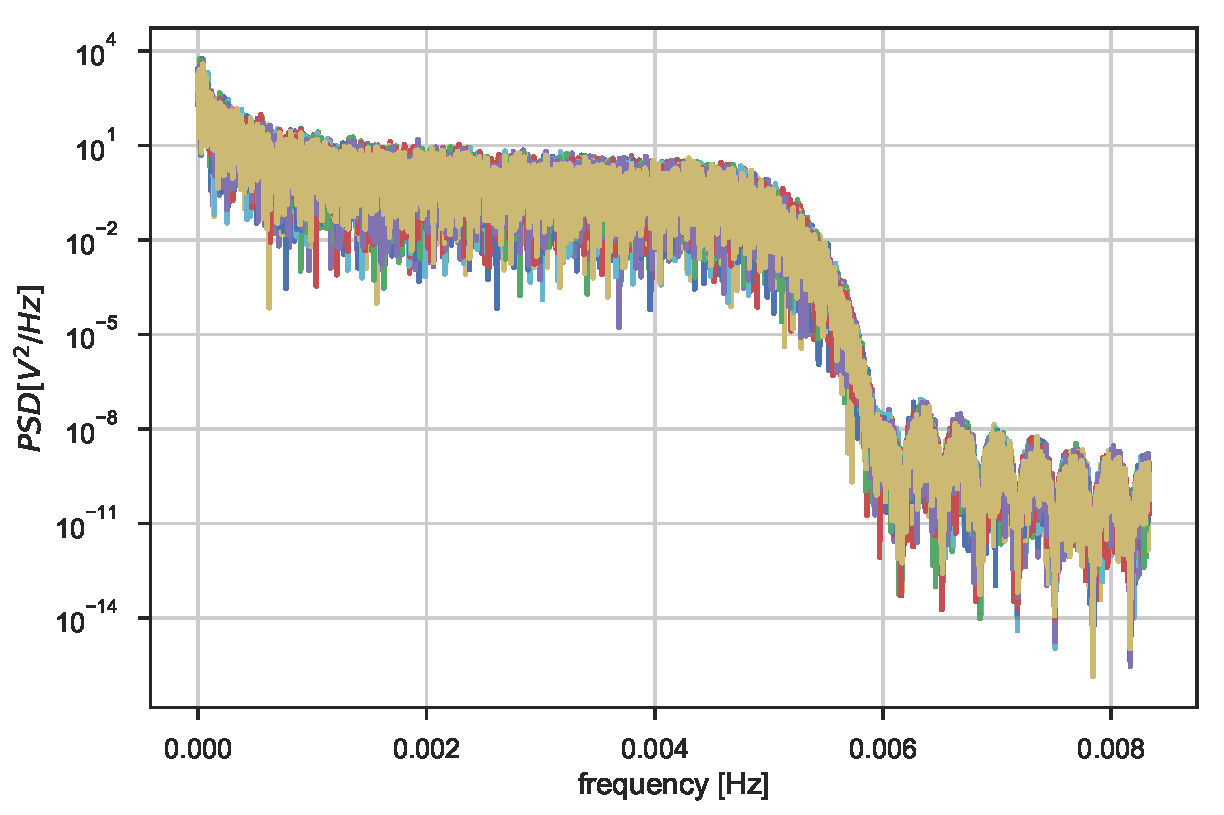
\includegraphics[width=\textwidth]{./sec/fig/periodogram.pdf}
%  \caption{Power spectral density}
%  \label{fig:fft1}
%\end{subfigure}%
%\begin{subfigure}{.5\textwidth}
%  \centering
%  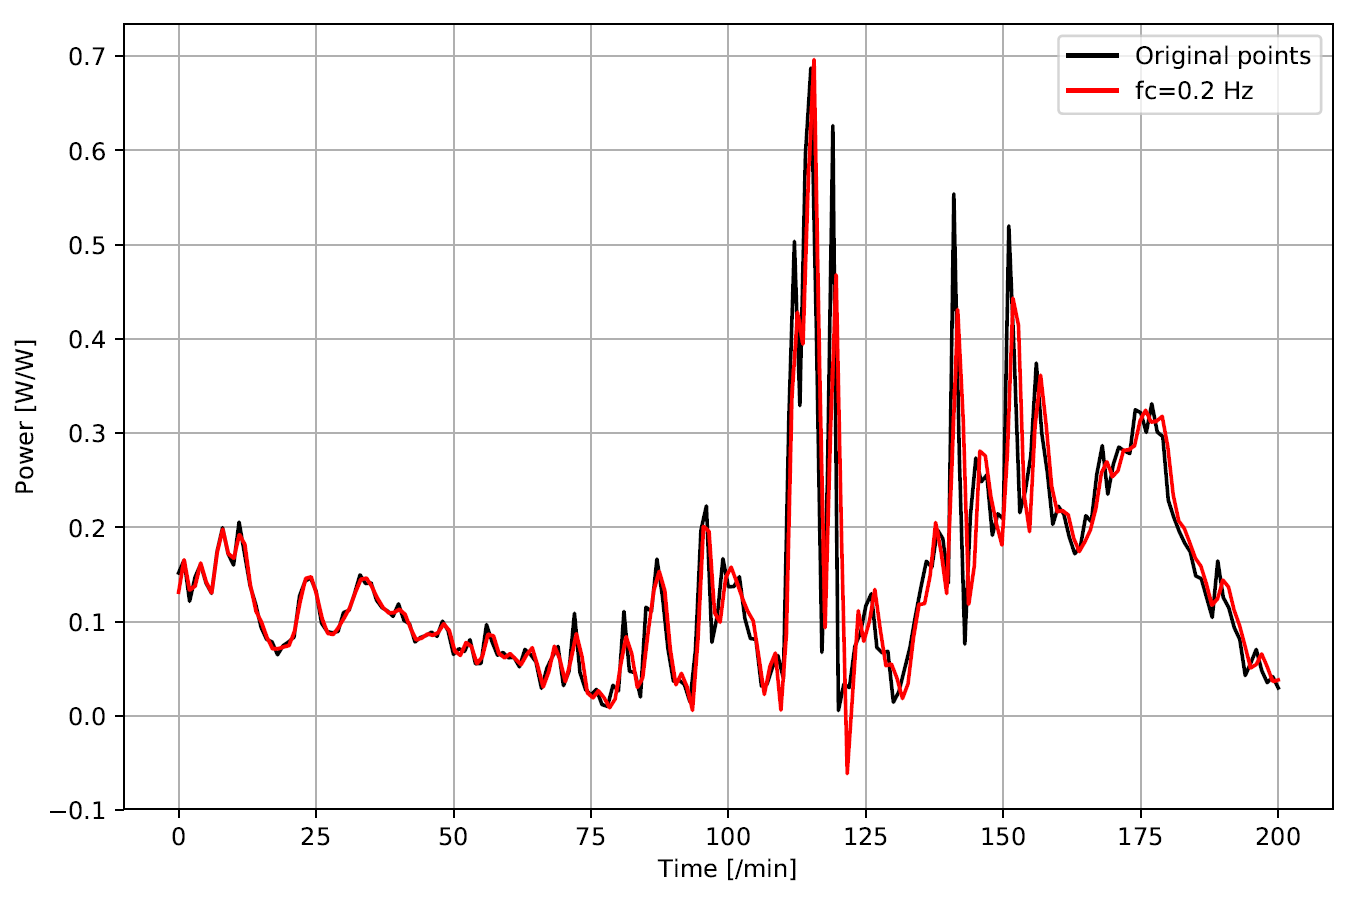
\includegraphics[width=\textwidth]{./sec/fig/fft2.png}
%  \caption{Filtered data with 0.2 Hz cut-off frequency}
%  \label{fig:fft2}
%\end{subfigure}
%\caption{Frequency domain interpretation of cut-off point}
%\label{fig:fft}
%\end{figure}

Fig. \ref{fig:fft} presents the data in frequency domain after the transformation from time to frequency domain. A Blackman window filter is used to remove the noise content in the wind power data. A smaller time window is chosen to demonstrate the changes. In fig. \ref{fig:fft}(A) the original data and data with 0.3 Hz cut-off frequency ($f_s$) is presented. Power spectral density (Welch-periodogram)of $x[n]$ is presented in fig. \ref{fig:fft}(B). 
The data is pre-processed for removing the noise content in the data during measurement. For this, a smoothing technique is used to smooth the data. Following that, a time to frequency domain transformation is performed. In this process, the data is passed through Blackman filter. The subsequent section explains the RBA$_\theta$ and the extraction of events from the original time-series power production.

\subsection{Improved Ramping Behaviour Algorithm}

RBA (Ramping Behvaiour Analysis) is a model to detect wind ramp events. Consider the wind power generation $w_t$ at discrete time $t$ and the consecutive measurement as $w_{t+1}$ where the balance is $w_{\Delta \;t}$. A finite variation $\Delta \; w$ therefore denoted as a ramp. Positive value of $\Delta \; w$ becomes a positive ramp and otherwise is denoted as a negative ramp. 
Thus a ramp event $\Delta \; w_s$ is defined as an event where a significant change in power generation takes place in a time period $\Delta \; t$. The significance is determined through the parameter $T$ that stands for an adjustable threshold to neglect $\Delta \; w$ values that are smaller than a set threshold $T$ as in  $\Delta \; w_s = \Delta \; w \quad | \Delta \; w > T $. A detailed explanation of RBA is presented in the \cite{ArticleNo1},\cite{ArticleNo2}. The mathematical expression for identification of peak points is presented in \eqref{eq:ramp1a}.
 
 
   \begin{figure}[!htbp]
    \centering
    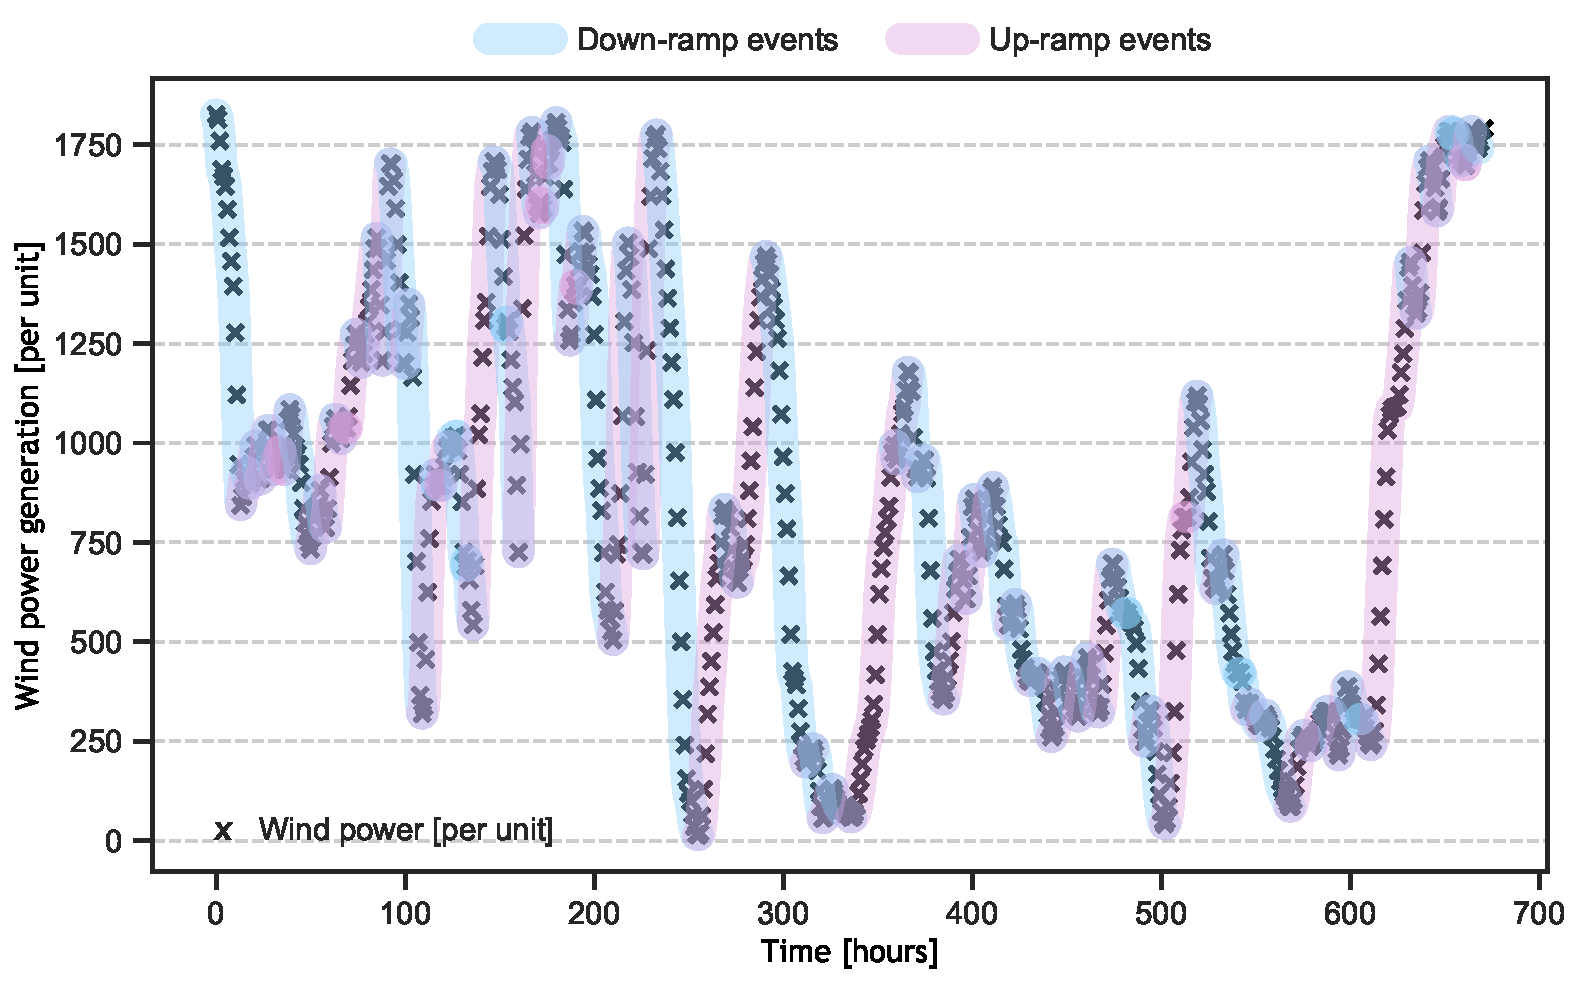
\includegraphics[width=0.9\textwidth]{./sec/fig/RBAevents.pdf}%RBAevents_final.pdf}
    \caption{Wind ramp detection with 5\% threshold}
    \label{fig:ramp_theta}
\end{figure}
% \begin{align} \label{eq:ramp}
%     \Delta \; w_s = \Delta \; w \quad | \Delta \; w > T
% \end{align}
The angle between the interval and the change in amplitude is denoted as $\theta$. It can be formulated as in \eqref{eq:ramp1}. An algorithmic description of the $RBA_\theta$ is presented in algorithm \ref{algo1}. The description includes two functions. The first one extract the events and the second one evaluates the number of occurrences of those events. The algorithm takes the input of time varying wind data (vector), the total length of the time period (scalar). Then the events are identified with respect to peak points and event characteristics: ramp-up, ramp-down, rise-time, fall-time, angle of the peak with respect to adjacent minima and persistence values are the results. The angle $\theta$ between two significant changes $\Delta \; w_s$ and $\Delta \; t$ is presented in \eqref{eq:ramp1b}. 


\begin{subequations} \label{eq:ramp1}
\begin{align}
    \textit{mean} \; ( \Delta w_{s}) & = \bigg( \frac{ w_{s,t} + w_{s, (t + \Delta \; t)}}{2} \bigg) \label{eq:ramp1a}\\
    \theta ( \Delta w_{s}) &= \arctan \; ( \Delta w_{s},  \Delta \; t) \label{eq:ramp1b}
\end{align}
\end{subequations}


%%%%%%%%%%%%%% RBA ALGORITHM
\begin{algorithm}[!htbp] 
\SetKwInOut{Input}{Input}
\SetKwInOut{Output}{Output}
\SetAlgoLined
\KwResult{$w_{s,t}, w_{s, (t+\Delta \; t)}, (t+ \Delta t), \Delta w_s,
 \theta(  \Delta w_s), \text{mean} (\Delta w_s)$, $\Delta w_s^f$,
  $\Delta t_s^f$, $(\theta (\Delta w_s))^f$, $\text{mean} (\Delta w_s^f)$}
\underline{function} $RBA_\theta$ \;
\Input{$ T, w_t \quad \in \mathsf{R}^+ $ }
$\Delta w = w_{ t + \Delta \; t } - w_t$ \;
\For{$i \leftarrow 1$ \textbf{to} \textit{length}( $ \Delta w $ )}{
\If{sign( $\Delta w[i]$ ) == sign( $\Delta w [i+1]$ ) }{
concatenate( $\Delta w$ )}
}
\For{$i \leftarrow 1$ \textbf{to} \textit{length}( $ \Delta w $) }{
\If{ $\Delta w > T$ }{
$\Delta w_s \leftarrow \Delta w$}
}
\For{$i \leftarrow$ \textbf{to} \textit{length}( $\Delta w_s$ ) }{
\If{sign( $\Delta w_s[i]$ ) == sign ( $\Delta w_s [i+1]$ )  }{
concatenate( $\Delta w_s$ )\\
events[i] $\leftarrow w_{s,t}, w_{s, (t + \Delta t)}, t, (t + \Delta t),
\Delta t_s, \theta (\Delta w_s), \text{mean} (\Delta w_s)$}
}
 \caption{$RBA_\theta$ algorithm pseudo code}
 \label{algo1}
\end{algorithm}
%%%%%%%%%%%%%%%%%%%%%%%%%%%%


The threshold $T$ was set to 0.01 or 5\% of the nominal capacity of the wind turbine. Fig. \ref{fig:ramp_theta} presents the resulting ramp event detection. The power production are marked with $x$ marks and ramp-up and ramp-down events are highlighted through blue and purple. Arrows present the scheme used to classify the events, for instance a long red arrow describes a long ramp-up event wherein there are two peak points considered as one significant up event. Note that the first ramp up event persisted for longer period in comparison to the second and third. Similarly the third ramp event persisted for longer period than the other. Clearly persistence values explain the length of an event and thereby indicates the severity. In other words, in a specific period of time if there exists multiple peak points with or without slight difference then the multiple points are counted as one event persisting over that time period.
Note that frequency and persistence are distinct from each other. While the frequency counts the number of occurrences of an event in the time-series data, the persistence values demonstrate how long an event has persisted with respect to time.

\begin{table}[!htbp]
\centering
\begin{tabular}{ccccccccc} \hline
Event & $w_s^t$ & $\Delta \; w_s (t+\Delta t)$ & $t$ & $t+\Delta t$ & $\Delta w_s^t$ & $\Delta t$ & $\theta \Delta w_s$ & $mean(\Delta w_s)$ \\ \hline
01 &	0.580	&	0.798	&	0.000	&	1.000	&	0.218	&	1.000	&	65.340	&	0.689	\\
02 &	0.691	&	0.336	&	14.000	&	123.000	&	-0.355	&	109.000	&	-1.868	&	0.514	\\
03 	&	0.482	&	0.684	&	872.000	&	914.000	&	0.201	&	42.000	&	2.743	&	0.583	\\
04 &	0.684	&	0.126	&	914.000	&	1083.000	&	-0.558	&	169.000	&	-1.891	&	0.405	\\
05 &	0.541	&	0.126	&	1012.000	&	1083.000	&	-0.415	&	71.000	&	-3.347	&	0.333	\\
06 &	0.126	&	0.367	&	1083.000	&	1150.000	&	0.241	&	67.000	&	2.063	&	0.246	\\
07 	&	0.215	&	0.683	&	1348.000	&	1466.000	&	0.468	&	118.000	&	2.270	&	0.449	\\
08 &	0.683	&	0.515	&	1466.000	&	1523.000	&	-0.168	&	57.000	&	-1.685	&	0.599	\\
09 &	0.522	&	0.291	&	1532.000	&	1589.000	&	-0.231	&	57.000	&	-2.320	&	0.407	\\
10	&	0.291	&	0.714	&	1589.000	&	1658.000	&	0.422	&	69.000	&	3.503	&	0.502	\\
\hline
\end{tabular}
\caption{RBA$_\theta$ parameters}
\label{tbl:rba1}
\end{table}

The frequency of occurrence is a measure to count these ramp events in the time horizon of the wind power data. Since this method identifies local peaks in the data with respect to the adjacent minimum point, the first ramp-up event ignores the first peak (at 0.16) and considers the peak at 0.20 in y-axis. Consequently the adjacent minimum point 0.13 is ignored and 0.12 is recorded. There is an overlap of the events at the meeting point this is because the event length includes both the starting and end point of the wind power data. In this way, events are aligned end-to-end. With that, $RBA_\theta$ identifies and counts the events while recording the event details at all stages. The table \ref{tbl:rba1} presents the RBA$_\theta$ parameters for 10 sample events.  

\subsection{RBA$_\theta$ Frequency and Persistence} \label{ss:persistence}
Frequency of an event can be defined as the number of times it occurs. Frequency of occurrences for $\Delta w_s$, $\Delta t$, $ \text{mean} \Delta w_s$, $\alpha \Delta w_s$ with corresponding ranges are evaluated. The ranges or bins are assumed to be linearly spaced between 1 and 100. The algorithmic representation for the RBA$_\theta$ frequency function is presented in algorithm \ref{algo2}.
The table \ref{tbl:freq1}  presents the start and end points for the event parameters for frequency evaluation. Input time series can be of different forms, for instance a triangular or step. For the former the persistence would be zero because there is only one peak for a time period. In case of the later there would be multiple points with or without slight variations with respect to a time period. 
Table \ref{tbl:freq2} presents the parameters and corresponding the frequency of occurrences of events.

\begin{algorithm}[!htbp] 
\SetKwInOut{Input}{Input}
\SetKwInOut{Output}{Output}
\SetAlgoLined
\Input{$\Delta w_s$, $\Delta t_s$, $(\theta (\Delta w_s))$, $\text{mean} (\Delta w_s)$}
\KwResult{$\Delta w_s^f$,
  $\Delta t_s^f$, $(\theta (\Delta w_s))^f$, $\text{mean} (\Delta w_s^f)$}
\For{bin$_1$=-1 $\ldots 1$}{
$w_{s,bin_1} $ 
}
\For {bin$_2$ = 1 $\ldots$ max $(\Delta t_s)$}{
$\Delta \; t_{s,bin_2}$
}
\For{bin$_3 = -90 \ldots 90$}{
$\theta ( \Delta w_{s, bin_3} )$ 
 }
%\For{$bin_3$ = (min ( mean} $(\Delta w_s))  \ldots $ max(mean $( \Delta w_s))$ }{
%$mean (\Delta w_{s, bin_3} $ 
% }
%%%%%%%%%%%%  bin3 and bin4 ? 
% frequency . what is a parameter?
\underline{function} frequency \\
\Input{param, bin} 
\For{ $i \leftarrow$ \textbf{to} \textit{length} (bin) }{
\For{ $k \leftarrow$ \textbf{to} \textit{length} (param)}{
\If{ param[k] $\leq$  bin[k+1]}{
$f[i] += 1$}
}}
\For{ $i \leftarrow$ \textbf{to} \textit{length} (bins)-1}{
\For{ $k \leftarrow$ \textbf{to} \textit{length} (param)}{
frequency[i] = f[i]
}}
$ \Delta w_{s}^f $ = frequency ($\Delta w_s , \Delta w_{s,bin_1} $) \\
$ \Delta t_{s}^f $ = frequency ($\Delta t_s , \Delta t_{s,bin_2}$) \\
$ \theta (\Delta w_{s}^f) $ = frequency ($ \theta (\Delta w_s , \Delta w_{s,bin_3})$) \\
$ mean (\Delta w_{s}^f) $ = frequency ($ mean (\Delta w_s , \Delta w_{s,bin_4})$) \\
 \caption{$RBA_\theta$ frequency function}
 \label{algo2}
\end{algorithm}


\begin{table}[!htbp]
\centering
\begin{tabular}{ccc} \hline
Event parameters 	& Starting point & Ending point \\ \hline
$\Delta w_s$ 			& -1 					& 01 					\\
$\Delta t$ 				& 01 					& max$(\Delta t)$ \\
mean$(\Delta w_s)$ & min(mean$(\Delta w_s)$) & max(mean$(\Delta w_s)$) \\
$\alpha (\Delta w_s)$ & -90$^o$ & 90$^o$ \\ \hline
\end{tabular}
\caption{Frequency measures of events with start and end points}
\label{tbl:freq1}
\end{table}



\begin{table}[!htbp]
\centering
\begin{tabular}{ccccccccc} \hline
Event & $\Delta w_s$ &  $\Delta w_s^f$  & $\Delta t$ & $\Delta t^f$ & $\theta \Delta w_s$ & $\theta \Delta w_s^f$ & mean($\Delta w_s)$ & mean($\Delta w_s^f$) \\ \hline
01	&	0.218	&	14	&	1	&	1	&	65.340	&	1	&	0.689	&	5	\\
02	&	-0.355	&	10	&	109	&	9	&	-1.868	&	167	&	0.514	&	5	\\
03	&	0.201	&	20	&	42	&	13	&	2.743	&	37	&	0.583	&	3	\\
04	&	-0.558	&	7	&	169	&	5	&	-1.891	&	167	&	0.405	&	9	\\
05	&	-0.415	&	4	&	71	&	16	&	-3.347	&	23	&	0.333	&	9	\\
06	&	0.241	&	18	&	67	&	17	&	2.063	&	159	&	0.246	&	4	\\
07	&	0.468	&	4	&	118	&	8	&	2.270	&	159	&	0.449	&	4	\\
08	&	-0.168	&	26	&	57	&	15	&	-1.685	&	167	&	0.599	&	2	\\
09	&	-0.231	&	16	&	57	&	15	&	-2.320	&	167	&	0.407	&	9	\\
10	&	0.422	&	9	&	69	&	12	&	3.503	&	37	&	0.502	&	3	\\
\hline
\end{tabular}
\caption{RBA$_\theta$ frequency of events}
\label{tbl:freq2}
\end{table}


The persistence can be defined as the act of continuing to exist past the usual time. Therefore the persistence event is a series of points that stays within the defined threshold value for longer than a predefined time limit. The algorithmic representation of persistence is presented in algorithm \ref{algo3}. The time period is chosen to be two days. In this period all the events extracted are sorted and the first event that has persisted for highest time is saved as a persistent event. The table \ref{tbl:p-rba} presents the persistence values for ten events. The persistence values for $w_{s,t}$ and $w_{s, t+ \Delta t}$ are presented through time $t$, time difference $t+ \Delta t$, mean and time difference $\Delta t$.

\begin{algorithm}[!htbp] 
\SetKwInOut{Input}{Input}
\SetKwInOut{Output}{Output}
\SetAlgoLined
\Input{ $mean, \Delta t$}
\KwResult{ $\overline{mean}, \overline{\Delta t}$}
periods=$t+1$ \\
bins= linspace(0,$t$,periods)  \\
t = length(filtered) \\
\For{$i$ in range(length(bins-1))}{
\For{$k$ in range(length($mean, \Delta t$))}{
\If{bins$_i <$ $mean_k , \Delta t_k$$<$ bins$_{i+1}$}{
sort ($\overline{mean}, \overline{\Delta t}$)
}}}
\caption{$RBA_\theta$ persistence function}
 \label{algo3}
\end{algorithm}

\begin{table}[!htbp]
\centering
\begin{tabular}{ccccccc} \hline
Event & $w_{s,t}$ &  $w_{s, t+ \Delta t}$  & $t$ & $t + \Delta t$ & mean & $\Delta t$ \\ \hline
01	&	0.453	&	0.302	&	100	&	477	&	0.378	&	377	\\
02	&	0.439	&	0.591	&	102	&	832	&	0.515	&	730	\\
03	&	0.265	&	0.416	&	1056	&	1389	&	0.340	&	333	\\
04	&	0.583	&	0.411	&	1624	&	1999	&	0.497	&	375	\\
05	&	0.452	&	0.302	&	100	&	477	&	0.377	&	377	\\
06	&	0.438	&	0.590	&	102	&	831	&	0.514	&	729	\\
07	&	0.276	&	0.428	&	1054	&	1392	&	0.352	&	338	\\
08	&	0.571	&	0.408	&	1622	&	1999	&	0.489	&	377	\\
09	&	0.482	&	0.331	&	94	&	466	&	0.406	&	372	\\
10	&	0.471	&	0.621	&	96	&	889	&	0.546	&	793	\\
\hline
\end{tabular}
\caption{RBA$_\theta$ persistence of events}
\label{tbl:p-rba}
\end{table}






\subsection{Rainflow Counting Cycle for Event extraction} \label{ssec:rainflow}
Rainflow counting algorithm \cite{downing1982simple} was developed to be used in the analysis of fatigue data in order to reduce a spectrum of varying stress into a set of simple stress reversals. The input to the algorithm is a simple series of peaks and valleys i.e., local maxima and minima, that form hysteresis loops. Closed loops are full cycles, and open loops are half cycles. The algorithm uses a change in slope as an indicator that the time series is going through a peak or valley. Only the magnitude of the peak or valley is then entered into the Rainflow counting algorithm.

\begin{table}[!htbp]
\centering
\begin{tabular}{ccc} \hline
Events & $w_s^t$ & Cycles \\ \hline
01	&	0.218	&	0.5\\
02	&	-0.355	&	0.5\\
03	&	0.201	&	1\\
04	&	-0.558	&	1\\
05	&	-0.415	&	0.5\\
06	&	0.241	&	0.5\\
07	&	0.468	&	0.5\\
08	&	-0.168	&	1\\
09	&	-0.231	&	1\\
10	&	0.422	&	0.5\\
\hline
\end{tabular}
\caption{Rainflow counting cycle for first ten events}
\label{tbl:rainflow}
\end{table}

It was implemented as presented in \cite{rinker2014including}. This algorithm is used to extract the cycles, with modifications to extract the starting and ending points of ramp events hence the time range, the starting and ending power of the events hence the amplitude, the angle of the event and the cycle with some minor modifications. A sample parameter values for the rainflow counting cycle is presented in the table \ref{tbl:rainflow}. The full cycles are presented as 1 and half-cycles as 0.5. For example, the events 3 and 4 have full cycles. 

\section{Time-series Prediction using Deep Learning }
\label{ssec:lstm}


%\begin{itemize}
%\item Describe Deep learning, RNN, LSTM 
%\item Describe optimizer
%\item 8 plots for prediction of each wind turbine, each plot original vs predicted.
%\end{itemize}

Recurrent neural networks (RNNs) might be less potent than feed-forward networks but they are applicable in some cases which require communication between each neuron as it is in our task.


LSTM is a specified RNN architecture, and it is one of the most applicable networks for forecast time series. RNN is possibly the closest network that mimics the human brain. As it can be understood from the term “long-short”, the aim of this network is to model temporal sequences and their long-term dependencies. LSTM uses stochastic gradient descent as an optimization tool. The reason behind RNN outperforms than feed-forward networks is it contains cyclic connections. Thanks to these connections it is easier to model sequence data \cite{sak2014long}.


\section{Spatial Markov Chain applications} \label{sec:markov}
The theory of spatial dynamics states that the power production from individual turbine can be quite different even though they are physically located in one farm and quite close to each other. The difference might arise from wake effect , terrain condition and other environmental effects. 
To capture this relation, a spatial dynamics approach has been considered. Specifically, spatial Markov chain model \cite{rey2001spatial,carle1997modeling}. In this section, a finite state spatial dynamics model is presented that is used to derive the transition matrix for the wind turbines in a wind farm. 
A Markov chain has a series of states $n$ which are mutually exclusive of each other thus applicable to discrete data-set. A transition matrix has transition probabilities from one state to another. The fig. \ref{fig:queen} presents the spacial relationship between wind turbines. The location information is presented in the table \ref{tbl:spatial}. The polygons are created using the GeoDa \cite{anselin2006geoda} program. 

\begin{figure}
\centering
\begin{subfigure}{.5\textwidth}
  \centering
  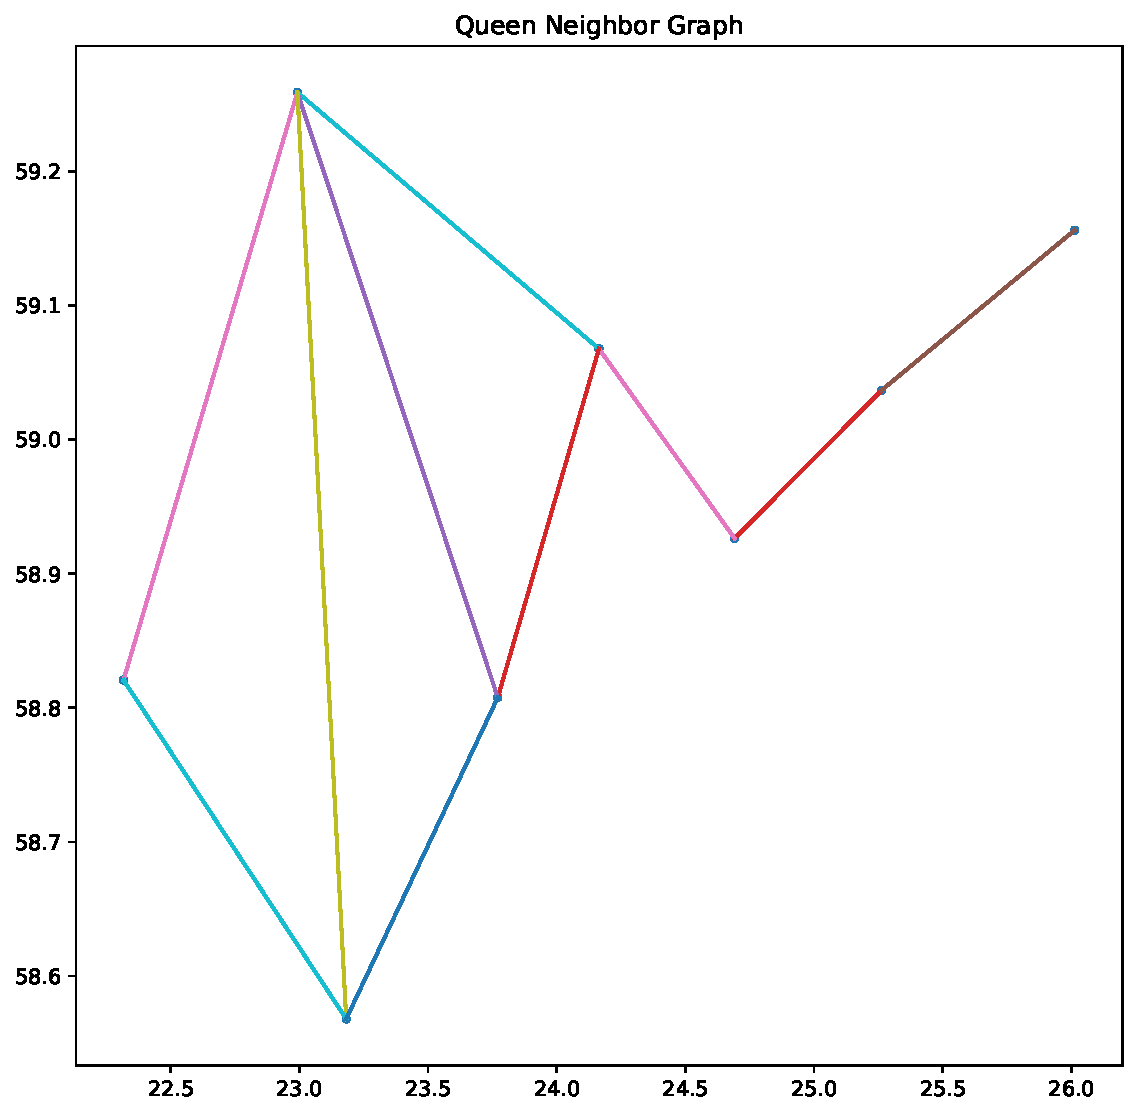
\includegraphics[width=\linewidth]{./sec/fig/queenrelationships.pdf}
 % \caption{A subfigure}
  \label{fig:sub1}
\end{subfigure}%
\begin{subfigure}{.5\textwidth}
  \centering
  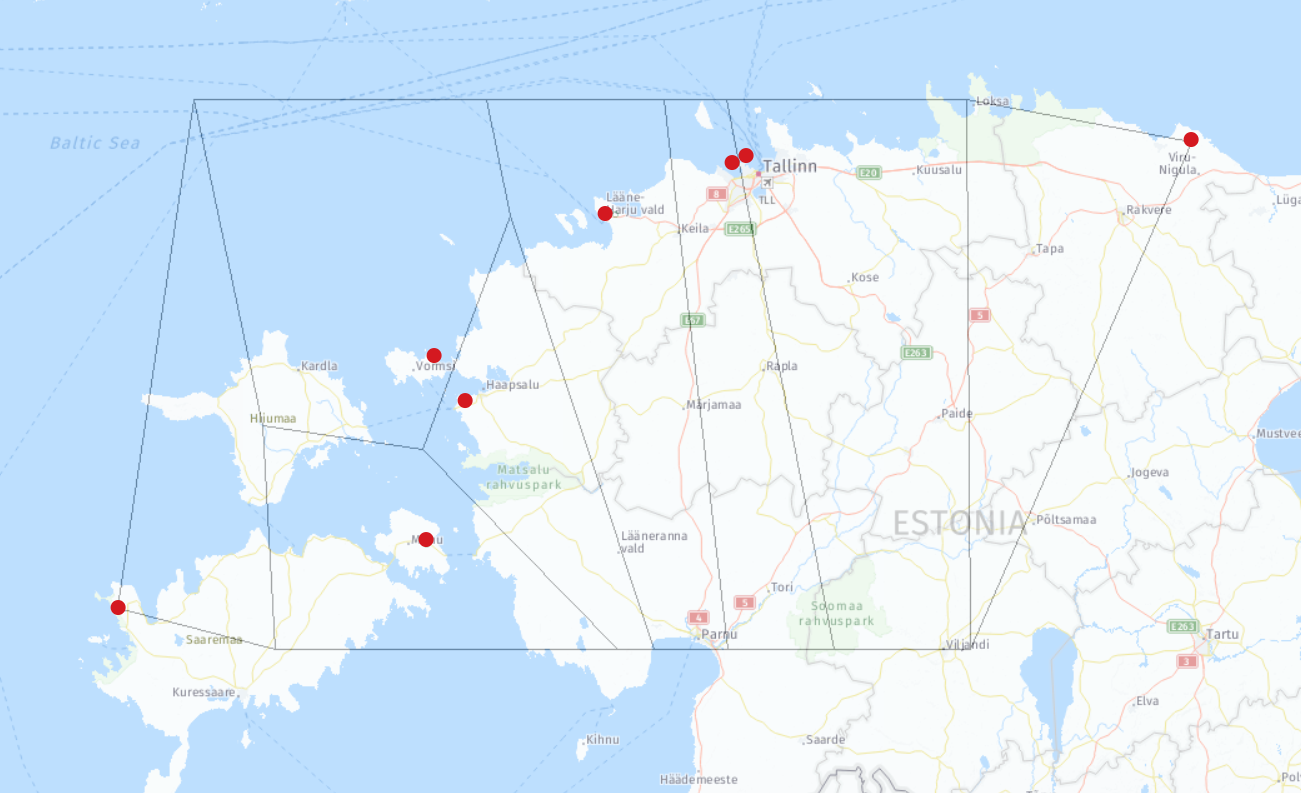
\includegraphics[width=\linewidth]{./sec/fig/thiessen_polygons.png}
 % \caption{A subfigure}
  \label{fig:sub2}
\end{subfigure}
\caption{Spatial relation between wind turbine locations: on left queens neighbor graph and on right the actual locations in Estonia}
\label{fig:queen}
\end{figure}


\begin{table}[!htbp]
\centering
\begin{tabular}{cccl} \hline
Wind turbine & Longitude		& Lattitude & Location\\ \hline
01	&	59.4784	&		24.6923	&	Paljassaare conservation area,Tallinn				\\
02	&	59.4646	&		24.6567	&	Kopli peninsula,Tallinn				\\
03	&	59.3416	&		24.1315	&	Paldiski, Harju county				\\
04	&	59.0257	&		23.3329	&	Norrby, Lääne county				\\
05	&	58.4434	&		21.9644	&	Kõruse, Saare county				\\
06	&	58.9245	&		23.4778	&	Rohuküla, Lääne county				\\
07	&	59.4953	&		26.6583	&	Iila, Lääne-Viru county				\\
08	&	58.5955	&		23.2965	&	Mõega, Saare county				\\ \hline
\end{tabular}
\caption{Location of wind turbines}
\label{tbl:spatial}
\end{table}

%\begin{itemize}
%\item why use spatial markov? pysal package
%\item Spatial and Lisa Markov description with references
%\item Location and queen plots
%\item results through tables or figures
%\end{itemize}


\subsection{Markov process}
A deterministic Markov chain has the following property

\begin{equation} \label{eq:m1}
P(X_{n+1}^t) \in A | X_0^t \ldots = x_n ) = P ( X^t_{n+1} \in A | X_n^t = x_n )
\end{equation}

In \ref{eq:m1} the Markov property of the future state $n+1$ depends only on the current state $n$ not the past state $n-1$. The process spread over all time $t_0 \leq t_1 \leq \ldots t_n \leq t_{n+1}$ and state space $x_0, \ldots x_n$. The transition kernel for the probability matrix can be expressed as in \ref{eq:m2}.

\begin{equation} \label{eq:m2}
P_{s,t} (x,A) := P(x_t \in A | X_s =x)
\end{equation}

The kernel generates transition probability value $A$ that the process takes at time $t$ given that at time $s$ the value was $x$. The transition matrix is expressed as $P(p(x,y))_{x,y \in s}$. The initial state is $P(X_0 =x)_{x \in s}$. The distribution at time $t=1$ is presented in \eqref{eq:m3}. One step transition probability is expressed in \eqref{eq:m4}. 

 \begin{align} 
P(X_1 =x) &= \sum_{x_0 \in S} P(X_0 = x_0) * P(X_1 =x | X_0 =x_0)  \\  \label{eq:m3}
p(x,y) & := P(X_{n+1} = y | X_n =x)   \\ \label{eq:m4}
\end{align}
  


\section{Scenario generation through spatial Markov transition matrices}
\label{sec:scen}


\begin{itemize}
\item why markov transition matrix to make scenarios
\item long and short term scenario
\item 4*4 matrix with 2 plots for short and 2 for long term scenarios with original data
\end{itemize}

%\section{Results}\label{results}
%
In this section we describe the results.

\section{Conclusion} \label{conclusion}
%%%%%%%%%%%%%%%%%%%%%%%%%%%
%
%		Conclusion
%
%%%%%%%%%%%%%%%%%%%%%%%%%%%

Here is the conclusion and future scope of RBA$_\theta \dotsc$



\bibliographystyle{unsrt}
\bibliography{citations}

\end{document}

